 \setlength{\baselineskip}{20pt}
% chapters/chapter06.tex
\chapter{一体化建模下的MaaS多阶段采纳意愿建模}\label{chap.integrated}

%==================================================================
\section{本章引论}\label{sec.int.intro}

第\ref{chap.staged}章已从``分阶段建模''的视角研究了MaaS多阶段采纳意愿。首先构建单次出行场景下的混合潜在分类模型刻画用户的转移意愿，进而计算转移意愿指数作为用户对MaaS``初始印象''的度量，并纳入下一套餐订阅阶段的混合潜在分类模型中捕捉用户对MaaS套餐的异质偏好，从而将两阶段相衔接。该框架可分别精细刻画两阶段的偏好异质性，有效辨识各阶段内的MaaS采纳的关键因素。然而，分阶段建模将两阶段先后、独立地进行模型估计，虽通过构建转移意愿指数将两阶段相衔接，但对两阶段间动态联系的刻画仍不充分。因此，本章仍聚焦研究内容（3），拟从``一体化建模''的视角对MaaS多阶段采纳意愿进行研究，旨在刻画两阶段间的动态联系，并在全周期视角下识别MaaS采纳的关键驱动因素。为此，首先简要分析分阶段建模框架的不足。

首先，分阶段建模以单向传递的``转移意愿指数''衔接两阶段，这意味着单次出行体验对套餐订阅的影响只能以一个事先计算、外生给定的标量传入，既无法回收两阶段参数间的相关性，也难以保证估计的一致性\citep{walkerGeneralizedRandomUtility2002}，缺乏统一的似然函数进行联合估计，难以在全周期视角下刻画MaaS采纳的关键驱动因素。

其次，分阶段建模隐含地假设用户的偏好类型在两阶段间保持不变，即无论是单次出行阶段的潜在类别，还是套餐订阅阶段的潜在类别，均在各自阶段内固定。然而，用户的行为状态可能在初次体验MaaS后发生改变。例如，对MaaS持谨慎态度、在单次出行阶段不愿转移的用户，可能因体验到显著的MaaS便利性而转向对MaaS更为积极的态度。这种跨阶段的行为状态转移是连接``初次体验''与``后续订阅''的关键环节，而既有文献（含第\ref{chap.staged}章）尚未对其建模，致使两阶段间的动态联系无法被定量刻画。

为弥补上述不足，本章提出一体化建模视角下的MaaS多阶段采纳意愿建模框架，其核心思想为，通过设计MaaS多阶段订阅隐马尔可夫模型（Hidden Markov Model, HMM），将受访者的行为状态贯穿于单次出行与套餐订阅两阶段，从而允许同一受访者的行为状态在两阶段间转变，进而在统一框架内同时刻画初始状态形成、跨阶段状态转移与两阶段的选择行为。具体而言，本章的研究思路可概括为三点：

\cp{1}针对联合估计中态度潜变量的识别与度量，沿用第\ref{chap.staged}章经探索性因子分析（EFA）与验证性因子分析（CFA）检验的五因子态度结构，构建MIMIC模型。以社会经济与出行模式属性为自变量解释各潜变量（结构模型），以有序Probit刻画潜变量与态度陈述的关系（测量模型），经极大似然估计后计算每位受访者的潜变量因子得分，作为HMM中刻画行为状态的潜变量。

\cp{2}针对多阶段采纳决策与跨阶段行为状态转移，构建贯穿两阶段的HMM，包含四个相互衔接的子模型：初始行为状态隶属模型刻画用户在单次出行阶段所处的初始状态，单次出行选择模型刻画各状态下用户是否转移至MaaS，跨阶段状态转移模型刻画用户在体验单次出行后向套餐订阅阶段的状态转移，套餐订阅选择模型刻画各状态下用户的套餐选择。四个子模型在统一的联合似然下同时估计，从而显式刻画两阶段间的动态联系。

\cp{3}针对一体化建模视角下与分阶段建模视角下的结果对比，分析两种建模范式在刻画MaaS采纳行为异质性与识别关键驱动因素上的差异。通过一体化建模可通过HMM模型构建的多阶段行为链条，识别MaaS多阶段全周期的采纳驱动因素，并给出面向全体用户的采纳驱动因素排序。此外，通过对比一体化建模与分阶段建模的估计结果，可厘清两种范式的适用边界，为第\ref{chap.optimization}章MaaS推广策略仿真中智能体多阶段采纳行为参数的选用提供依据。

在数据基础方面，本章与第\ref{chap.staged}章采用同一份两步式SP调查数据，其调查设计、样本特征与态度量表已于第\ref{chap.staged}章及附录~D中详细阐述，故本章不再赘述数据采集过程，而将重点置于一体化模型的构建与估计结果分析。

%==================================================================
\section{多指标多原因模型构建}\label{sec.int.mimic}

为纳入潜变量刻画用户的态度异质性，本节沿用\ref{subsec.staged.bundle.lv}节中识别到的性价比偏好、技术接受度、计划性偏好、环保意识与现状满意度五个潜变量。由于HMM模型的标定过程计算复杂性过高，难以应用混合选择模型框架将结构模型与测量模型引入到HMM模型中同步估计，故本节采用两步法对模型进行估计。首先，构建多指标多原因（Multiple Indicators Multiple Causes, MIMIC）模型，同时刻画潜变量的形成机制与潜变量对态度陈述的影响\citep{joreskogEstimationModelMultiple1975}，为后续HMM中刻画行为状态提供潜变量因子得分。

MIMIC模型由结构方程与测量方程两部分构成\citep{joreskogEstimationModelMultiple1975}：结构方程以可观测的个体相关变量为原因解释各潜变量，测量方程则以有序Probit刻画潜变量与其对应态度陈述（指标）之间的关系。MIMIC模型的结构如图~\ref{fig.int.mimic}所示。下面依次介绍结构方程、测量方程，以及似然函数与因子得分的计算。

\begin{figure}[H]
  \centering
  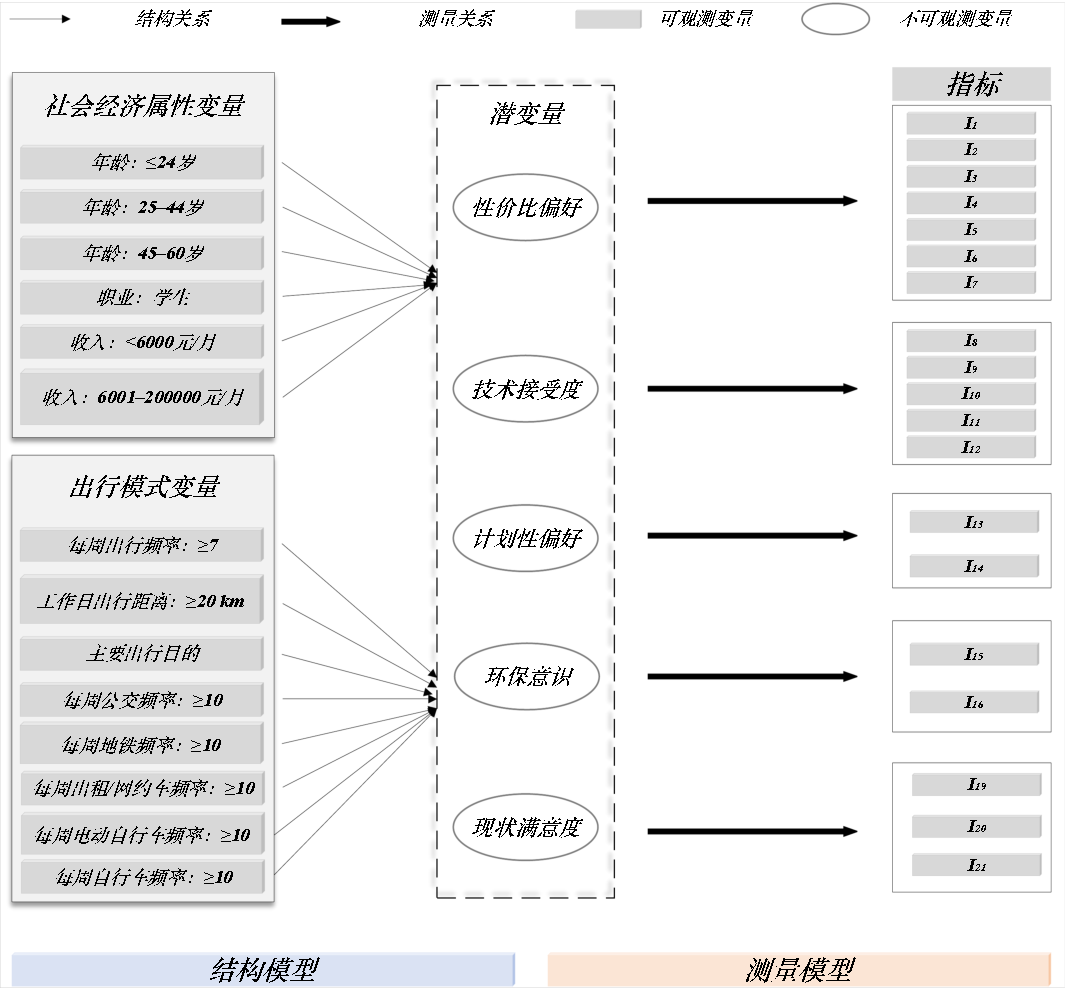
\includegraphics[width=\textwidth]{figures/ch6/中文版/MIMIC_framework.pdf}
  \bicaption{MIMIC模型结构}{Structure of the MIMIC model.}
  \label{fig.int.mimic}
\end{figure}

\subsection{结构方程构建}\label{subsec.int.structural}

结构方程以可观测的受访者自身相关的变量解释各潜变量，以刻画社会经济与出行模式属性对态度的塑造。对潜变量$f$与受访者$n$，结构方程为：
\begin{equation}\label{eq.int.structural}
a_{n,f} = \sum_{k=1}^{K} \beta_{k,f}\, Z_{n,k} + \sigma_f\, \varepsilon_{n,f},\qquad \varepsilon_{n,f}\sim \mathcal{N}(0,1),
\end{equation}
式中，$a_{n,f}$为受访者$n$在潜变量$f$上的取值；$Z_{n,k}$为$K$个观测变量中的第$k$个；$\beta_{k,f}$为$Z_{n,k}$对潜变量$f$的系数；$\sigma_f$为潜变量$f$的尺度参数；$\varepsilon_{n,f}$为服从标准正态分布的随机扰动项。与第\ref{chap.staged}章类似，本章从两类属性中选取观测变量。一是社会经济属性（年龄、收入与职业），二是出行模式属性（每周出行频率、每周出行距离、主要出行目的与各方式的出行频率）。值得注意的是，结构方程的主要目的在于计算潜变量因子得分，因此本章尽可能纳入更多的观测变量以解释潜变量的异质性。

\subsection{测量方程构建}\label{subsec.int.measurement}

测量方程刻画潜变量与其对应态度指标之间的关系，与\ref{subsec.staged.bundle.lv}节类似，本章仍沿用有序Probit模型\citep{dalyUsingOrderedAttitudinal2012}。设$I_{n,j}\in\{1,2,3,4,5\}$为受访者$n$对指标$j$的响应，$f(j)$为指标$j$所载荷的潜变量，则观测到响应为$c$的概率为：
\begin{equation}\label{eq.int.measurement}
P\!\left(I_{n,j}=c\mid a_{n,f(j)}\right)=\Phi\!\left(\frac{\tau_c^{(f(j))}-\alpha_j-\lambda_j\, a_{n,f(j)}}{\sigma_j}\right)-\Phi\!\left(\frac{\tau_{c-1}^{(f(j))}-\alpha_j-\lambda_j\, a_{n,f(j)}}{\sigma_j}\right),
\end{equation}
式中，$\Phi(\cdot)$为标准正态分布的累积分布函数；$\alpha_j$为指标$j$的截距；$\lambda_j$为潜变量$f(j)$对指标$j$的载荷，为待估参数；$\sigma_j$为指标层面的尺度参数；$\tau_c^{(f)}$为潜变量$f$的第$c$个阈值。为识别模型，设$\tau_0^{(f)}=-\infty$、$\tau_5^{(f)}=+\infty$、$\tau_1^{(f)}=0$，并将其余阈值参数化为累积增量$\tau_c^{(f)}=\tau_{c-1}^{(f)}+\delta_c^{(f)}$，其中$\delta_c^{(f)}>0$（$c\in\{2,3,4\}$）；同时，对每个潜变量，将其首个载荷指标锚定为$\lambda=1$、$\alpha=0$、$\sigma=1$。

\subsection{似然函数与潜变量计算}\label{subsec.int.likelihood}

综合结构方程与测量方程，MIMIC模型中受访者$n$的似然贡献为全部观测指标在五维潜变量向量$\boldsymbol{a}_n$上的联合概率密度积分：
\begin{equation}\label{eq.int.mimicLn}
L_n=\int_{\boldsymbol{a}_n} f_I\!\left(\boldsymbol{I}_n\mid \boldsymbol{a}_n;\alpha,\lambda,\sigma_I,\tau\right)\cdot f_a\!\left(\boldsymbol{a}_n\mid \boldsymbol{Z}_n;\beta,\sigma_a\right)\, d\boldsymbol{a}_n,
\end{equation}
\begin{equation}\label{eq.int.mimicfI}
f_I\!\left(\boldsymbol{I}_n\mid \boldsymbol{a}_n\right)=\prod_{f\in F}\prod_{j\in J_f}\prod_{c\in C} P\!\left(I_{n,j}=c\mid a_{n,f}\right)^{\delta(I_{n,j}=c)},
\end{equation}
\begin{equation}\label{eq.int.mimicfa}
f_a\!\left(\boldsymbol{a}_n\mid \boldsymbol{Z}_n\right)=\prod_{f\in F}\frac{1}{\sigma_f}\,\phi\!\left(\frac{a_{n,f}-\sum_{k=1}^{K}\beta_k^{(f)} Z_{n,k}}{\sigma_f}\right),
\end{equation}
式中，$f_I(\cdot)$为全部测量方程的联合似然函数，$f_a(\cdot)$为全部结构方程的联合概率密度；$F$为潜变量集合，$J_f$为潜变量$f$对应的态度陈述集合，$C=\{1,2,3,4,5\}$为李克特量表的有序取值集合；$\delta(I_{n,j}=c)$为指示函数，当受访者$n$对态度陈述$j$选取测量值$c$时取1、否则取0；$\phi(\cdot)$为一元标准正态密度函数。

由于式\refeq{eq.int.mimicLn}中的积分无解析解，本节基于模拟极大似然估计思想，借助Python开源工具包Biogeme~3.3.2\citep{bierlaireShortIntroductionBiogeme2023}，以500次模拟极大似然抽样（Maximum Simulated Likelihood Sampling, MSLS）最大化对数似然之和$\sum_n \ln L_n$对模型进行估计。估计完成后，即可根据受访者的社会经济及出行模式属性，计算其五个潜变量的取值$\overline{a}_{n,f}$，并将其作为态度属性纳入\ref{sec.int.hmm}节的HMM，从而在不引入内生性的前提下刻画受访者态度对行为状态的影响。

%==================================================================
\section{基于隐马尔可夫模型的多阶段采纳意愿建模}\label{sec.int.hmm}

在计算得到每位受访者的潜变量取值后，本节进一步介绍基于隐马尔可夫模型（Hidden Markov Model, HMM）的MaaS多阶段采纳意愿建模框架，以刻画受访者在单次出行与套餐订阅两阶段的使用意愿偏好及阶段间的行为状态转移。HMM被广泛用于刻画出行行为中的状态转移\citep{chenHowIncomeSatisfaction2023,yuHighorderHiddenMarkov2023}，适用于本章所关注的MaaS多阶段采纳问题，其由不可观测的潜在状态序列与观测到的行为选择序列构成，潜在状态序列刻画受访者在不同阶段作出MaaS采纳选择时所处的、不可观测的潜在行为状态，而观测到的行为选择序列则为受访者在特定状态各阶段下作出的选择，对应不同的偏好结构。

具体而言，HMM在统一的建模框架内刻画四个相互衔接的过程：\cp{1}受访者在单次出行阶段所处的初始行为状态（\ref{subsec.int.init}小节）；\cp{2}确定的初始行为状态如何影响其单次出行选择（\ref{subsec.int.choice1}小节）；\cp{3}单次出行的选择后，行为状态是否发生转变（\ref{subsec.int.trans}小节）；\cp{4}转移后的（可能为新的）行为状态如何决定其套餐订阅选择（\ref{subsec.int.choice2}小节）。四个子模型在单一联合似然下同时估计（\ref{subsec.int.joint}小节）。本章将HMM设定为含$K$个潜在行为状态，状态集合记为$\mathcal{S}=\{1,2,\ldots,K\}$。图~\ref{fig.int.framework}为HMM的总体结构。

\begin{figure}[H]
  \centering
  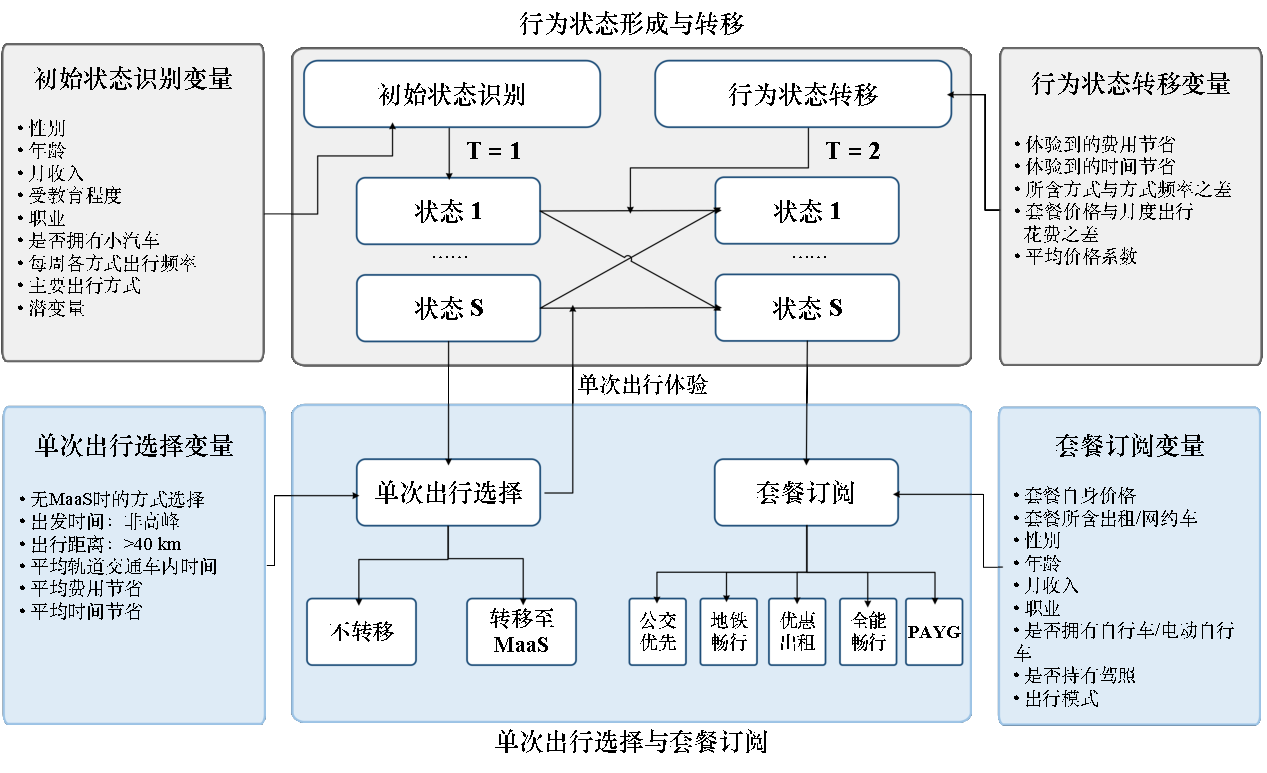
\includegraphics[width=\textwidth]{figures/ch6/中文版/HMM_framework.pdf}
  \bicaption{一体化建模下MaaS多阶段采纳意愿建模总体框架}{Overall framework for integrated modeling of multi-stage MaaS adoption intention.}
  \label{fig.int.framework}
\end{figure}

值得注意的是，关于四个子模型效用函数的具体形式，采用迭代式的设定流程，即先估计仅含状态特定ASC的基准模型，再向四个子模型的效用函数中逐步加入其他变量。在此过程中，将显著性较低的变量剔除并在其他子模型中试验。最终，依据调整后$R^2$、AIC、BIC等指标及变量显著性，确定四个子模型的效用函数的具体设定。下面依次介绍各子模型。

\subsection{初始行为状态隶属模型}\label{subsec.int.init}

受访者在初次接触MaaS并进行对应的采纳决策（即单次出行情境下的MaaS多模式出行服务采用决策）前处于处于某一不可观测的初始状态，该状态影响其首个行为阶段的行为偏好，并可能展现出不同的采纳意愿与行为选择。为此，构建初始行为状态隶属模型以刻画受访者初始状态的形成机制，帮助理解单次出行阶段的偏好异质性及后续的行为状态转移过程。采用以状态$s=1$为参照的多项Logit设定，受访者$n$处于状态$s$的概率为：
\begin{equation}\label{eq.int.init}
P\!\left(S_n^{st}=s\right)=\frac{\exp\!\left(V_n^{\mathrm{init},s}\right)}{\sum_{s'\in\mathcal{S}}\exp\!\left(V_n^{\mathrm{init},s'}\right)},\qquad s\in\mathcal{S},
\end{equation}
式中，$P\!\left(S_n^{st}=s\right)$为受访者$n$在作单次出行选择时处于状态$s$的概率，$V_n^{\mathrm{init},s}$为处于状态$s$的效用，设定为：
\begin{equation}\label{eq.int.initV}
V_n^{\mathrm{init},s}=\alpha_0^{s}+\sum_{k=1}^{K_{\mathrm{ind}}}\alpha_k^{s}\, X_{n,k}+\sum_{f\in F}\alpha_f^{s}\,\overline{a}_{n,f},
\end{equation}
式中，$\boldsymbol{X}_{n,k}$为第$k$个受访者自身的社会经济与出行模式变量，用以刻画由个体自身特征塑造的异质偏好，$K_{\mathrm{ind}}$为受访者自身有关的变量的总数。$\overline{a}_{n,f}$为受访者$n$的潜变量$f$的计算值，刻画潜在态度对行为状态的影响；$\alpha_0^{s}$为状态特定常数；$\alpha_k^{s}$与$\alpha_f^{s}$为待估的状态特定系数。

\subsection{单次出行阶段选择模型}\label{subsec.int.choice1}

在识别受访者的初始状态后，进一步刻画不同行为状态下受访者如何作出初次接触MaaS，即单次出行阶段的MaaS多模式出行服务采纳选择。本章将单次出行选择建模为二元决策，即在提供MaaS多模式服务的情境下，受访者是否从原有的出行方案转移到使用MaaS。为此，采用二元Logit模型，处于状态$s$下的受访者$n$在单次出行情境下转移至MaaS的概率为：
\begin{equation}\label{eq.int.choice1}
P\!\left(Y_{n}^{st}=1\mid S_n^{st}=s\right)=\frac{\exp\!\left(V_{n}^{st,s}\right)}{\exp\!\left(V_{n}^{st,s}\right)+1},\qquad s\in\mathcal{S},
\end{equation}
式中，在状态$s$下受访者$n$转移至MaaS的效用为：
\begin{equation}\label{eq.int.choice1V}
V_{n}^{st,s}=\mathrm{ASC}^{st,s}+\sum_{k}\beta_{k}^{st,s}\, X_{n,k}^{st},
\end{equation}
式中，$\boldsymbol{X}_{n}^{st}$为单次出行情境层面的属性，包括单次出行情境下选择的MaaS多模式出行服务带来的费用节省与时间节省、轨道车内时间，以及无MaaS多模式出行服务情境下的选择结果等变量；$\mathrm{ASC}^{st,s}$为状态特定的方案常数；$\beta_{k}^{st,s}$为状态$s$下属性$X_{n,k}^{st}$的系数，用以刻画不同状态下受访者对单次出行情境属性的异质偏好。

\subsection{跨阶段行为状态转移模型}\label{subsec.int.trans}

在单次出行阶段做出是否使用MaaS的多模式出行服务决策后，受访者形成了对MaaS的初始态度与偏好，因此其之后针对MaaS的行为状态可能在单次出行选择后发生改变，进而影响其套餐订阅选择。例如，一名持谨慎态度的受访者在单次出行阶段可能处于不愿采纳MaaS新兴出行服务的状态，但在体验MaaS后，可能因感受到费用节省与便捷而转向更积极的状态，从而提高其订阅MaaS套餐的可能性。为此，本小节对由单次出行阶段向套餐订阅阶段的行为状态转移加以建模，以理解受访者跨阶段的MaaS采纳行为变化。

具体而言，在行为状态转移过程中，受访者的行为状态可能由单次出行阶段的状态$S_n^{st}$转移至套餐订阅阶段的状态（可能不同）$S_n^{bs}$，其转移受受访者偏好、单次出行阶段所体验到的MaaS多模式出行服务质量，以及套餐订阅阶段的套餐属性共同影响。因此，将状态转移过程构建为条件于单次出行阶段状态$S_n^{st}$的多项Logit模型，进而确定转移向套餐订阅阶段状态$S_n^{bs}$的概率如下：
\begin{equation}\label{eq.int.trans}
P\!\left(S_n^{bs}=s'\mid S_n^{st}=s\right)=\frac{\exp\!\left(V_n^{\mathrm{trans},s\to s'}\right)}{\sum_{s''\in\mathcal{S}}\exp\!\left(V_n^{\mathrm{trans},s\to s''}\right)},\qquad s,s'\in\mathcal{S},
\end{equation}
式中，$P\!\left(S_n^{bs}=s'\mid S_n^{st}=s\right)$为受访者$n$由单次出行阶段的状态$s$转移至套餐订阅阶段的状态$s'$的概率，$V_n^{\mathrm{trans},s\to s'}$为该转移的效用，设定为：
\begin{equation}\label{eq.int.transV}
V_n^{\mathrm{trans},s\to s'}=G_0^{s\to s'}+\sum_{k=1}^{K_{\mathrm{trans}}}G_k\, W_{n,k}^{\mathrm{trans}},
\end{equation}
式中，$G_0^{s\to s'}$为单次出行和套餐订阅两阶段状态间特定的转移截距，刻画由状态$s$向状态$s'$转移的基准倾向；$W_{n,k}^{\mathrm{trans}}$为受访者$n$的第$k$个转移变量；$G_k$为相应系数。重点考虑三类转移变量：其一，单次出行阶段所体验到的MaaS多模式出行服务质量（如MaaS选项相对原方式在受访者层面平均的费用节省与时间节省），刻画单次出行阶段的体验如何影响状态转移；其二，套餐属性与受访者出行模式的匹配程度，包括套餐所含方式的服务水平与受访者主要出行方式频次的匹配程度、套餐价格与受访者当前月度出行花费的匹配程度等，刻画套餐与出行模式的匹配程度如何影响状态转移；其三，套餐的平均价格系数，刻画套餐的性价比如何影响状态转移。

\subsection{套餐订阅阶段选择模型}\label{subsec.int.choice2}

在经历单次出行选择并转移至（可能新的）行为状态后，受访者在转移后的行为状态下做出第二阶段的MaaS套餐订阅选择。与\ref{subsec.int.choice1}小节的单次出行选择模型相对应，套餐订阅选择模型刻画各状态下受访者的套餐选择。关于模型形式，考虑到嵌套Logit在本章的联合估计中无法收敛，故采用多项Logit。以PAYG为参照方案，处于状态$s$的受访者$n$选择套餐$b$的概率为：
\begin{equation}\label{eq.int.choice2}
P\!\left(Y_{n}^{bs}=b\mid S_n^{bs}=s\right)=\frac{\exp\!\left(V_{n,b}^{bs,s}\right)}{\sum_{b'\in\mathcal{A}^{bs}}\exp\!\left(V_{n,b'}^{bs,s}\right)},\qquad b\in\mathcal{A}^{bs},\; s\in\mathcal{S},
\end{equation}
式中，$Y_n^{bs}$为受访者$n$的套餐订阅选择，$V_{n,b}^{bs,s}$为在行为状态$s$下受访者$n$选择套餐$b$的效用，设定为：
\begin{equation}\label{eq.int.choice2V}
V_{n,b}^{bs,s}=\mathrm{ASC}_{b}^{bs,s}+\sum_{k}\gamma_{b,k}^{bs,s}\, X_{n,b,k}^{bs},
\end{equation}
式中，$\mathrm{ASC}_{b}^{bs,s}$为状态与套餐特定的常数；$\gamma_{b,k}^{bs,s}$为状态$s$下套餐属性$X_{n,b,k}^{bs}$的系数；$X_{n,b,k}^{bs}$为影响受访者$n$选择套餐$b$的第$k$个属性。

在效用函数设定上，主要考虑两方面：一是套餐属性，包括套餐价格与所含方式；二是受访者本身属性，包括社会经济与出行模式属性。其中，套餐价格变量加入到全部四种MaaS套餐的效用函数中，以刻画不同状态的受访者对套餐价格的差异化权衡；套餐中可用的出租/网约车变量加入到公交优先与地铁畅行两套餐的效用函数，以考察补充性出租/网约车服务对这两种公交导向套餐吸引力的影响。个体相关变量（性别、年龄、收入、受教育程度、职业、是否持照、是否拥车，以及各方式的每周出行频率）则加入到全部四种MaaS套餐的效用函数，刻画不同特征与出行模式的受访者在套餐订阅上的差异化偏好。

\subsection{联合似然函数与模型标定}\label{subsec.int.joint}

\textbf{（1）联合似然函数}

若将MIMIC模型与HMM模型进行联合估计，则完整似然为受访者的选择对$(Y_{n}^{st},Y_{n}^{bs})$的联合概率与其潜变量因子得分$\boldsymbol{a}_n$的联合概率密度在五维潜变量向量上积分、并对所有可能的状态路径求和，其计算负担在当前条件下不可行，故本章不对MIMIC与HMM作完全联合估计，而采用两阶段标定策略。因此，HMM的似然仅包含\ref{subsec.int.init}至\ref{subsec.int.choice2}小节所述的四个子模型。由于单次出行阶段状态$S_n^{st}$与套餐订阅阶段状态$S_n^{bs}$均不可观测，受访者$n$在某一情境下观测到的选择对$(Y_{n}^{st},Y_{n}^{bs})$的联合概率，须对全部$K^2$条可能的状态路径$(s,s')\in\mathcal{S}\times\mathcal{S}$求和，即：
\begin{equation}\label{eq.int.joint}
\begin{aligned}
P\!\left(Y_{n}^{st},Y_{n}^{bs}\right)=\sum_{s\in\mathcal{S}}\sum_{s'\in\mathcal{S}}
& \, P\!\left(S_n^{st}=s\right)\cdot P\!\left(Y_{n}^{st}\mid S_n^{st}=s\right)\\
& \cdot P\!\left(S_n^{bs}=s'\mid S_n^{st}=s\right)\cdot P\!\left(Y_{n}^{bs}\mid S_n^{bs}=s'\right),
\end{aligned}
\end{equation}
式中，四个条件概率分别由式\refeq{eq.int.init}、式\refeq{eq.int.choice1}、式\refeq{eq.int.trans}与式\refeq{eq.int.choice2}给出。HMM的完整对数似然为全部``受访者$\times$情境''观测上$\log P(Y_{n,t}^{st},Y_{n,t}^{bs})$之和，其中下标$t$标识受访者$n$所贡献的情境：
\begin{equation}\label{eq.int.loglik}
\mathcal{LL}_{\mathrm{HMM}}=\sum_{n=1}^{N}\sum_{t=1}^{T_n}\log P\!\left(Y_{n,t}^{st},Y_{n,t}^{bs}\right),
\end{equation}
式中，$N$为受访者数，$T_n$为受访者$n$的情境对数。

\textbf{（2）模型标定设置}

MIMIC模型与HMM模型均借助Python开源工具包Biogeme~3.3.2\citep{bierlaireShortIntroductionBiogeme2023}估计。MIMIC模型以500次MHLS抽样最大化模拟对数似然；HMM模型则最大化式\refeq{eq.int.loglik}的对数似然。在数据组织上，因两模型的似然结构不同，其数据组织也不同：对MIMIC模型，每位受访者仅贡献1条观测（25条态度陈述在SP实验中仅作答一次），共得1242条个体层面观测；对HMM模型，须将每位受访者的单次出行选择与其对应的套餐订阅选择两两配对，以完整观测两阶段间的行为转移，故共得27360条观测。由于每位受访者贡献多条情境对，本章报告在受访者层面聚类的稳健标准误，以校正同一受访者跨情境的决策的相关性。

%==================================================================
\section{模型结果分析}\label{sec.int.result}

本节报告并分析一体化建模框架下MIMIC模型的估计结果（\ref{subsec.int.res.mimic}小节）、HMM模型的估计结果（\ref{subsec.int.res.hmm}）。其中，HMM模型的结果分为从初始行为状态形成到套餐订阅选择建模等4个子模型的估计结果。

\subsection{MIMIC模型估计结果}\label{subsec.int.res.mimic}


在分析具体的参数估计结果之前，简要分析MIMIC模型的总体拟合情况，结果如表~\ref{tab.int.mimic.fit}所示。

MIMIC模型共估计132个参数，最终对数似然值为$-28239.92$，模型初始对数似然值为$-44012.50$，McFadden $\rho^2$为0.358、调整后McFadden $\rho^2$为0.355，AIC与BIC分别为$56743.85$与$57420.28$。表明模型能够较好地拟合受访者潜变量形成以及潜变量对态度陈述的影响。结构模型与测量模型的估计结果分别如下。

{
\small
\begin{longtable}{lc}
\bicaption{MIMIC模型总体拟合优度}{Overall goodness-of-fit statistics for the MIMIC model.}
\label{tab.int.mimic.fit} \\
\toprule
统计量 & 数值 \\
\midrule
\endfirsthead
\multicolumn{2}{l}{\small（续表~\ref{tab.int.mimic.fit}）}\\
\toprule
统计量 & 数值 \\
\midrule
\endhead
\midrule
\multicolumn{2}{r}{\small 续下页}\\
\endfoot
\bottomrule
\endlastfoot
观测数 & 1242 \\
估计参数个数 & 132 \\
零模型对数似然 & $-44012.50$ \\
最终对数似然 & $-28239.92$ \\
似然比检验 & $31545.16$ \\
McFadden $\rho^2$ & 0.358 \\
调整后McFadden $\rho^2$ & 0.355 \\
AIC & $56743.85$ \\
BIC & $57420.28$ \\
\end{longtable}
}

\textbf{（1）结构模型估计结果}

结构模型估计结果如表~\ref{tab.int.mimic.structural}所示。就年龄而言，以60岁以上为参照，其余三个年龄段的受访者对五个潜变量的系数均显著为正，介于1.06与2.46之间，说明60岁以下受访者在五个态度维度上的态度得分均高于老年参照组。就收入而言，以高收入组（$>$20000元/月）为参照，中低收入受访者在除计划性偏好外的潜变量上得分更高。关于出行模式变量对潜变量的影响，结果显示每周出行频率超过7次的受访者在性价比偏好、技术接受度、计划性偏好和现状满意度上均显著为正，每周公交出行频率超过10次的受访者在环保意识和现状满意度上显著为正，说明依赖公交出行的受访者更关注环境保护，并对现有出行状况更为满意。每周出行频率超过7次（0.155）与每周公交出行频率超过10次（0.063）的受访者对当前出行状况更为满意，这可能得益于北京公共交通系统较为发达，出行频繁、依赖公交者往往拥有较满意的出行体验。总体而言，受访者社会经济属性和出行模式变量对五个潜变量的影响略有差异，但大多显著影响均符合预期。

更多细节见表~\ref{tab.int.mimic.structural}。

\begin{landscape}
{
\footnotesize
\setlength{\tabcolsep}{4pt}
\begin{longtable}{L{0.20\linewidth}C{0.14\linewidth}C{0.14\linewidth}C{0.14\linewidth}C{0.14\linewidth}C{0.14\linewidth}}
\bicaption{MIMIC结构模型估计结果（括号内为稳健t值）}{Estimation results of the MIMIC structural model (robust $t$-values in parentheses).}
\label{tab.int.mimic.structural} \\
\toprule
观测变量 & 性价比偏好 & 技术接受度 & 计划性偏好 & 环保意识 & 现状满意度 \\
\midrule
\endfirsthead
\multicolumn{6}{l}{\footnotesize（续表~\ref{tab.int.mimic.structural}）}\\
\toprule
观测变量 & 性价比偏好 & 技术接受度 & 计划性偏好 & 环保意识 & 现状满意度 \\
\midrule
\endhead
\midrule
\multicolumn{6}{r}{\footnotesize 续下页}\\
\endfoot
\bottomrule
\endlastfoot
\multicolumn{6}{L{0.90\linewidth}}{\textit{社会经济属性}} \\*
年龄：$\leq$24             & 2.458 (7.60)***  & 1.521 (6.32)***  & 1.685 (6.27)***  & 1.056 (3.20)***  & 1.493 (6.42)*** \\
年龄：25--44               & 2.203 (7.06)***  & 1.368 (6.17)***  & 1.621 (6.28)***  & 1.154 (3.56)***  & 1.360 (6.20)*** \\
年龄：45--60               & 2.108 (6.85)***  & 1.226 (5.01)***  & 1.747 (6.25)***  & 1.314 (3.69)***  & 1.385 (5.60)*** \\
职业：学生                 & $-0.140$ ($-0.81$) & $-0.172$ ($-1.27$) & 0.009 (0.08)   & 0.181 (1.22)     & 0.014 (0.13)    \\
收入：$<$6000元/月         & 0.692 (3.11)***  & 0.398 (2.10)**   & 0.252 (1.49)     & 0.759 (2.78)***  & 0.274 (1.66)*   \\
收入：6001--20000元/月     & 0.638 (3.02)***  & 0.390 (2.10)**   & 0.204 (1.36)     & 0.657 (2.47)**   & 0.345 (2.16)**  \\
\midrule
\multicolumn{6}{L{0.90\linewidth}}{\textit{出行模式属性}} \\*
每周出行频率：$\geq$7      & 0.142 (2.75)***  & 0.119 (3.20)***  & 0.090 (2.65)***  & 0.049 (1.03)     & 0.155 (4.54)*** \\
每周出行距离：$\geq$20km   & 0.075 (1.68)*    & 0.018 (0.57)     & 0.050 (1.64)     & 0.076 (1.87)*    & 0.040 (1.35)    \\
出行目的：通勤             & 0.098 (0.62)     & 0.119 (1.23)     & 0.201 (2.06)**   & 0.212 (1.58)     & 0.052 (0.56)    \\
每周公交频率：$\geq$10     & $-0.005$ ($-0.11$) & 0.046 (1.40)   & 0.005 (0.18)     & 0.093 (2.16)**   & 0.063 (2.23)**  \\
每周地铁频率：$\geq$10     & 0.072 (1.57)     & 0.039 (1.20)     & 0.007 (0.25)     & $-0.005$ ($-0.12$) & 0.023 (0.81)  \\
每周出租/网约车频率：$\geq$10 & $-0.002$ ($-0.06$) & $-0.018$ ($-0.45$) & $-0.027$ ($-0.87$) & 0.060 (1.30) & 0.037 (1.30)  \\
每周电单车频率：$\geq$10   & $-0.132$ ($-2.50$)** & 0.068 (1.77)* & $-0.058$ ($-1.61$) & 0.007 (0.14) & $-0.012$ ($-0.33$) \\
每周自行车频率：$\geq$10   & 0.021 (0.44)     & $-0.010$ ($-0.31$) & 0.001 (0.03)   & 0.044 (0.99)     & 0.049 (1.59)    \\
\midrule
潜变量标准差 $\sigma_f$    & 1.189 (13.22)*** & 0.860 (15.63)*** & 0.523 (2.10)**   & 1.198 (11.72)*** & 0.700 (7.22)*** \\
\end{longtable}

{\footnotesize 注：$^{***}$、$^{**}$、$^{*}$分别表示在1\%、5\%、10\%水平下显著；年龄、收入的参照组分别为60岁以上、20000元/月以上。}
}
\end{landscape}

\textbf{（2）测量模型估计结果}

测量模型估计结果如表~\ref{tab.int.mimic.measure}所示。估计结果从三个方面证实了潜变量结构的有效性：其一，全部载荷系数均为正且在1\%水平下显著，量级介于0.621与1.132之间；其二，每个潜变量的三个响应阈值增量均为正且高度显著，确保有序Probit的阈值单调递增、满足识别要求；其三，指标层尺度参数因指标而异且均高度显著，反映19条指标响应离散程度的异质性。综上，测量模型验证了从结构模型中识别的潜变量对受访者态度陈述的影响，进一步说明潜变量结构的有效性。

{
\small
\setlength{\tabcolsep}{4pt}
\begin{longtable}{C{0.10\linewidth}C{0.26\linewidth}C{0.26\linewidth}C{0.26\linewidth}}
\bicaption{MIMIC测量模型估计结果（括号内为稳健t值）}{Estimation results of the MIMIC measurement model (robust $t$-values in parentheses).}
\label{tab.int.mimic.measure} \\
\toprule
相关指标 & 系数 & 截距 & 标准差 \\
\midrule
\endfirsthead
\multicolumn{4}{l}{\small（续表~\ref{tab.int.mimic.measure}）}\\
\toprule
相关指标 & 系数 & 截距 & 标准差 \\
\midrule
\endhead
\midrule
\multicolumn{4}{r}{\small 续下页}\\
\endfoot
\bottomrule
\endlastfoot
\multicolumn{4}{L{0.88\linewidth}}{\textbf{性价比偏好}（阈值增量：0.883 (11.39)***、1.105 (17.50)***、1.252 (20.80)***）} \\*
$I_1$    & 1（固定）        & 0（固定）          & 1（固定）        \\
$I_2$    & 0.778 (14.08)*** & 0.432 (2.43)**     & 1.114 (17.22)*** \\
$I_3$    & 0.621 (14.48)*** & 0.557 (4.02)***    & 1.017 (18.74)*** \\
$I_4$    & 0.789 (12.53)*** & 0.555 (2.78)***    & 1.053 (15.95)*** \\
$I_5$    & 0.864 (15.76)*** & 0.229 (1.33)       & 1.091 (17.04)*** \\
$I_6$    & 0.909 (16.46)*** & 0.011 (0.06)       & 1.037 (16.70)*** \\
$I_7$    & 0.837 (12.96)*** & 0.423 (2.04)**     & 1.263 (15.45)*** \\
\midrule
\multicolumn{4}{L{0.88\linewidth}}{\textbf{技术接受度}（阈值增量：0.682 (13.90)***、0.981 (23.47)***、1.082 (26.68)***）} \\*
$I_8$    & 1（固定）        & 0（固定）          & 1（固定）        \\
$I_9$    & 0.958 (13.20)*** & 0.320 (1.92)*      & 0.998 (21.25)*** \\
$I_{10}$ & 0.999 (15.12)*** & $-0.100$ ($-0.64$) & 0.847 (20.64)*** \\
$I_{11}$ & 1.132 (14.58)*** & $-0.322$ ($-1.78$)* & 0.751 (16.81)*** \\
$I_{12}$ & 1.108 (13.98)*** & $-0.363$ ($-1.99$)** & 0.872 (18.24)*** \\
\midrule
\multicolumn{4}{L{0.88\linewidth}}{\textbf{计划性偏好}（阈值增量：0.625 (8.62)***、0.830 (10.00)***、0.887 (10.14)***）} \\*
$I_{13}$ & 1（固定）        & 0（固定）          & 1（固定）        \\
$I_{14}$ & 0.691 (5.14)***  & 0.561 (2.25)**     & 0.938 (24.24)*** \\
\midrule
\multicolumn{4}{L{0.88\linewidth}}{\textbf{环保意识}（阈值增量：0.961 (12.15)***、1.167 (16.05)***、1.238 (18.25)***）} \\*
$I_{15}$ & 1（固定）        & 0（固定）          & 1（固定）        \\
$I_{16}$ & 0.945 (22.32)*** & 0.265 (2.47)**     & 0.983 (19.53)*** \\
\midrule
\multicolumn{4}{L{0.88\linewidth}}{\textbf{现状满意度}（阈值增量：0.744 (12.09)***、1.006 (17.88)***、1.234 (20.49)***）} \\*
$I_{19}$ & 1（固定）        & 0（固定）          & 1（固定）        \\
$I_{20}$ & 0.981 (11.33)*** & $-0.136$ ($-0.62$) & 1.187 (22.17)*** \\
$I_{21}$ & 0.677 (9.57)***  & 0.396 (2.21)**     & 0.958 (23.49)*** \\
\end{longtable}

{\footnotesize 注：$^{***}$、$^{**}$、$^{*}$分别表示在1\%、5\%、10\%水平下显著。}
}

\subsection{隐马尔可夫模型估计结果}\label{subsec.int.res.hmm}

结合MIMIC模型的模型标定结果，进一步计算每一受访者的潜变量得分，进一步将其纳入到HMM模型的标定过程。本小节分析HMM模型的估计结果。四个子模型的完整估计结果如表~\ref{tab.int.hmm}所示，括号内为稳健t值。下文将从总体拟合、初始行为状态识别、单次出行选择、跨阶段行为状态转移以及套餐订阅选择五个方面对HMM模型的估计结果进行分析。

\textbf{（1）状态数选择与总体拟合}

关于行为状态数量的选取，针对行为状态数量$K=2-4$的模型分别进行标定。然而，行为状态数量$K=3$与$K=4$的模型均无法收敛，且在$K=2$的模型中，模型的整体拟合程度较好，且具有较好的可解释性。综上，选取$K=2$作为HMM模型的最优状态数。$K=2$HMM模型的最终对数似然值为$-51639.19$，初始模型对数似然值为$-64662.29$，调整后McFadden $\bar{\rho}^2$为0.200，表明模型能够较好地解释受访者从初始行为状态形成到套餐订阅选择的联合决策过程。AIC与BIC分别为$103456.40$与$104187.70$。关于模型识别出的两个行为状态，根据受访者处于两行为状态在四个子模型中的决策偏好将其命名：第一个状态（表~\ref{tab.int.hmm}第二列）受访者在单次出行与套餐订阅决策中对费用更为敏感，故命名为``费用敏感型''；第二个状态（表~\ref{tab.int.hmm}第三列）受访者在单次出行阶段决策以及跨阶段行为状态转移中展现出对时间更为敏感的倾向，故命名为``时间敏感型''。后对这两种状态的形成过程、单次出行选择、跨阶段行为状态转移以及套餐订阅选择进行分析。

\clearpage
{
\small
\setlength{\tabcolsep}{3pt}
\begin{longtable}{@{}L{6.2cm}C{3.5cm}C{3.5cm}@{}}
\bicaption{HMM模型估计结果（括号内为稳健t值）}{Estimation results of the HMM (robust $t$-values in parentheses).}\label{tab.int.hmm} \\
\toprule
变量 & 费用敏感型 & 时间敏感型 \\
\midrule
\endfirsthead
\multicolumn{3}{l}{\small（续表~\ref{tab.int.hmm}）}\\
\toprule
变量 & 费用敏感型 & 时间敏感型 \\
\midrule
\endhead
\midrule
\multicolumn{3}{r}{\small 续下页}\\
\endfoot
\bottomrule
\endlastfoot

\multicolumn{3}{l}{\textbf{初始行为状态隶属模型}} \\*
ASC                                  & ——                & $-3.880$ ($-14.40$)*** \\*
女性                                 & ——                & 0.697 (12.40)***       \\*
年龄：25--44                         & ——                & $-0.009$ ($-0.15$)     \\*
年龄：$>$60                          & ——                & $-5.000$ ($-8.28$)***  \\*
收入：$<$6000元/月                   & ——                & 0.167 (1.27)           \\*
收入：6001--20000元/月               & ——                & 0.775 (6.35)***        \\*
受教育程度：本科及以上               & ——                & 0.608 (9.51)***        \\*
职业：学生                           & ——                & $-0.166$ ($-2.30$)**   \\*
拥车                                 & ——                & 0.221 (3.64)***        \\*
每周公交频率：$\geq$10               & ——                & $-0.240$ ($-10.70$)*** \\*
每周地铁频率：$\geq$10               & ——                & 0.436 (17.60)***       \\*
每周出租/网约车频率：$\geq$10        & ——                & $-0.168$ ($-5.51$)***  \\*
每周电单车频率：$\geq$10             & ——                & 0.272 (10.50)***       \\*
主要出行方式：租赁汽车               & ——                & 0.424 (5.19)***        \\*
主要出行方式：共享单车               & ——                & 0.826 (11.20)***       \\*
性价比偏好                           & ——                & $-0.066$ ($-2.14$)**   \\*
技术接受度                           & ——                & 0.466 (10.10)***       \\*
计划性偏好                           & ——                & 0.301 (3.25)***        \\*
环保意识                           & ——                & $-0.378$ ($-9.47$)***  \\*
现状满意度                           & ——                & 0.150 (2.58)***        \\
\addlinespace[2pt]
\multicolumn{3}{l}{\textbf{单次出行选择模型}} \\*
ASC：MaaS                            & $-2.050$ ($-9.74$)***  & 1.920 (10.20)***       \\*
无MaaS时的选择：公共交通             & 2.920 (14.90)***       & 3.590 (1.60)           \\*
无MaaS时的选择：出租/网约车          & $-0.009$ ($-0.05$)     & 1.030 (3.47)***        \\*
出发时间：非高峰                     & $-0.257$ ($-3.47$)***  & $-0.074$ ($-0.35$)     \\*
出行距离：$>$40km                    & $-6.210$ ($-9.20$)***  & 0.328 (0.99)           \\*
平均轨道交通车内时间                     & $-0.020$ ($-7.16$)***  & $-0.037$ ($-4.93$)***  \\*
平均费用节省（相对无MaaS选择，元）   & 0.459 (4.45)***        & 0.050 (0.74)           \\*
平均时间节省（相对无MaaS选择，min）  & $-0.017$ ($-0.29$)     & 0.143 (0.19)           \\
\addlinespace[2pt]
\multicolumn{3}{l}{\textbf{状态转移模型}} \\*
转移截距（$\to$时间敏感型）          & $-0.419$ ($-1.76$)*    & 0.027 (0.13)           \\*
体验到的费用节省（元）               & \multicolumn{2}{c}{$-0.006$ ($-5.47$)***}      \\*
体验到的时间节省（min）              & \multicolumn{2}{c}{0.005 (4.03)***}            \\*
所含方式与公交频率之差               & \multicolumn{2}{c}{$-0.294$ ($-5.74$)***}      \\*
所含方式与地铁频率之差               & \multicolumn{2}{c}{$-0.186$ ($-2.51$)**}       \\*
所含方式与自行车频率之差             & \multicolumn{2}{c}{0.220 (3.66)***}            \\*
所含方式与出租车频率之差             & \multicolumn{2}{c}{$-0.181$ ($-4.22$)***}      \\*
套餐价格与月度出行花费之差           & \multicolumn{2}{c}{0.018 (7.22)***}            \\*
平均价格系数                         & \multicolumn{2}{c}{0.318 (2.12)**}             \\
\addlinespace[2pt]
\multicolumn{3}{l}{\textbf{套餐订阅选择模型}} \\*
\multicolumn{3}{l}{\textit{方案特定常数}} \\*
ASC：公交优先                        & 1.320 (7.69)***        & $-0.271$ ($-2.05$)**   \\*
ASC：地铁畅行                        & 1.160 (5.31)***        & $-0.967$ ($-6.03$)***  \\
\multicolumn{3}{l}{\textit{套餐属性}} \\*
价格（公交优先、地铁畅行，百元）     & $-0.235$ ($-3.14$)***  & 0.015 (0.84)           \\*
价格（优惠出租、全能畅行，百元）     & $-0.024$ ($-2.23$)**   & 0.015 (0.84)           \\*
出租/网约车里程（公交优先、地铁畅行，百公里） & $-0.067$ ($-0.39$) & $-0.213$ ($-3.42$)*** \\
\multicolumn{3}{l}{\textit{公交优先}} \\*
女性                                 & 0.075 (0.85)           & $-0.323$ ($-7.06$)***  \\*
年龄：$>$60                          & 0.349 (1.34)           & 1.490 (7.38)***        \\*
收入：$<$6000元/月                   & 0.159 (1.33)           & $-0.063$ ($-1.01$)     \\*
职业：学生                           & 0.294 (2.75)***        & $-0.121$ ($-2.05$)**   \\*
自行车/电单车拥有                    & 0.232 (2.68)***        & 0.273 (5.02)***        \\*
每周公交频率：$\geq$10               & 0.863 (15.50)***       & 0.120 (4.41)***        \\
\multicolumn{3}{l}{\textit{地铁畅行}} \\*
收入：6001--20000元/月               & 0.387 (5.98)***        & $-3.790$ ($-1.84$)*    \\*
每周出行距离：$\geq$20km             & 0.069 (2.14)**         & 0.060 (2.58)***        \\*
每周地铁频率：$\geq$10               & 1.010 (16.70)***       & 0.333 (14.30)***       \\*
主要多模式出行：公交+共享单车        & 0.371 (4.10)***        & 0.015 (0.22)           \\
\multicolumn{3}{l}{\textit{优惠出租}} \\*
年龄：45--60                         & 0.784 (6.74)***        & $-4.970$ ($-7.98$)***  \\*
周末出行距离：$\geq$20km             & 0.036 (1.76)*          & $-0.253$ ($-2.29$)**   \\*
每周出租/网约车频率：$\geq$10        & 1.380 (8.39)***        & $-2.260$ ($-6.15$)***  \\
\pagebreak
\multicolumn{3}{l}{\textbf{套餐订阅选择模型（续）}} \\*
\multicolumn{3}{l}{\textit{套餐属性（续）}} \\*
\multicolumn{3}{l}{\textit{全能畅行}} \\*
月度出行花费：$>$1000元              & $-0.044$ ($-0.63$)     & 0.102 (2.14)**         \\*
主要出行方式：私家车                 & 0.402 (6.01)***        & 0.560 (2.60)***        \\
\multicolumn{3}{l}{\textit{PAYG}} \\*
受教育程度：本科及以上               & 2.270 (4.36)***        & 0.412 (6.18)***        \\*
持驾照                               & $-4.820$ ($-2.09$)**   & 0.488 (8.02)***        \\*
月度出行花费：$>$1000元              & $-0.044$ ($-0.63$)     & 0.102 (2.14)**         \\
\addlinespace[2pt]
\multicolumn{3}{l}{\textbf{模型概况}} \\*
样本数                               & \multicolumn{2}{c}{27360}              \\
初始对数似然值                       & \multicolumn{2}{c}{$-64662.29$}        \\
最终对数似然值                         & \multicolumn{2}{c}{$-51639.19$}        \\
估计参数个数                         & \multicolumn{2}{c}{89}                 \\
似然比检验                           & \multicolumn{2}{c}{$26046.20$}         \\
调整后McFadden $\rho^2$              & \multicolumn{2}{c}{0.200}              \\
AIC                                  & \multicolumn{2}{c}{$103456.40$}        \\
BIC                                  & \multicolumn{2}{c}{$104187.70$}        \\
\end{longtable}

{\footnotesize 注：$^{***}$、$^{**}$、$^{*}$分别表示在1\%、5\%、10\%水平下显著；``——''表示以费用敏感型为参照、相应系数归一化为0；状态转移模型仅设定转移至时间敏感型的效用、转移至费用敏感型的效用归一化为0。}
}

\textbf{（2）初始行为状态及其决定因素}

就受访者作单次出行选择前的初始状态而言，以费用敏感型为参照状态，ASC显著为负（$-3.880$）表明受访者更可能起始于费用敏感型，这与MaaS文献的既有结论一致：货币成本是MaaS采纳最常见的障碍\citep{kimComparativeAnalysisUsers2021,kriswardhanaGenerationalDifferencesPreferences2025}。就社会经济属性而言，女性（0.697）、收入6001-20000元/月的中等收入者（0.775）与本科及以上受教育者（0.608）更可能初始为时间敏感型状态，这可能因上述群体的时间压力相对更大，故在出行决策中对时间比对费用更为敏感；相反，60岁以上者（$-5.000$）与学生（$-0.166$）更可能为费用敏感型，这可能是因为其时间压力相对较小、对费用更为敏感。

就出行模式属性而言，公交与地铁的对比尤为鲜明：每周公交频率$\geq$10 的受访者（$-0.240$）初始更不可能处于时间敏感型，而每周地铁频率$\geq$10的受访者（0.436）则相反。值得注意的是，出行模式变量对初始状态形成的影响可能源于两个方面：一方面是正向的影响，即地铁通常被视为较公交更省时的方式，其高效性促使使用者形成看重时间的决策取向；另一方面则源于样本自身的出行习惯，即习惯乘坐公交的出行者本身在出行选择中更为在意出行费用。这种两方面的影响同样适用于其余出行模式变量，例如每周电动自行车频率$\geq$10的受访者（0.272）、以共享单车为主要出行方式的受访者（0.826）与拥有私人小汽车的受访者（0.221）均更可能形成时间敏感型的初始状态，不仅反映了这些灵活、按需出行方式的在节省出行时间上的吸引力，也反映了选择这些出行者本身偏重时间的生活方式。

就MIMIC模型测算的的态度潜变量而言，技术接受度（0.466）对初始状态为时间敏感型的影响最大，计划性偏好（0.301）与现状满意度（0.150）同样正向促进出行者初始形成时间敏感型的行为状态，这可能因为针对以上态度潜变量获得较高的分的受访者乐于组织并优化其出行体验，从而更倾向于看重时间的决策风格；相反，性价比偏好（$-0.066$）与环保意识（$-0.378$）的系数为负，即具有较高性价比偏好和环保意识的受访者更倾向于进入费用敏感型的初始行为状态。就初始状态分布而言，模型估计表明63.4\%的受访者起始于费用敏感型、36.6\%起始于时间敏感型，说明多数受访者在决策中以费用为先，而仍有一部分受访者以时间为先。

\textbf{（3）单次出行阶段的偏好异质性}

本部分总结两状态在单次出行阶段的异质行为模式。首先，两种行为状态下受访者的决策偏好最直观的差异体现在针对转向MaaS多模式出行服务的常数（ASC）上，即费用敏感型ASC为$-2.050$、时间敏感型ASC为1.920，说明在其他属性相同时，费用敏感型受访者倾向于拒绝在单次出行阶段使用MaaS多模式出行服务，而时间敏感型受访者倾向于采纳MaaS。从选择结果的概率分布来看，有21.7\%的费用敏感型受访者在单次出行阶段选择转向MaaS多模式出行服务，然而，却有80.9\%的时间敏感型受访者选择转向MaaS多模式出行服务，进一步说明两状态在单次出行阶段的决策偏好存在显著差异。MaaS多模式出行服务带来的费用节省与时间节省系数的标定结果进一步揭示了这一行为差异背后的机理。针对费用敏感型行为状态，平均费用节省系数显著为正（0.459），说明对出行费用的考量主导该状态的决策，即MaaS出行服务节省的出行费用越多，费用敏感型受访者越可能选择MaaS；而时间敏感型状态下，费用节省的标定系数不显著，表明费用节省在其决策中作用并不显著。与此相对，平均轨道交通车内时间的系数在时间敏感型（$-0.037$）中较费用敏感型（$-0.020$）更强地为负，表明时间敏感型受访者对MaaS多模式出行服务的出行时间更为敏感。

就无MaaS情境下受访者选择的既有出行方式的影响而言，估计结果呈现出明显的状态异质性。在费用敏感型状态下，无MaaS时本会选择公共交通的受访者更可能转移至采用MaaS多模式出行服务（2.920），说明在MaaS多模式无缝集成下，MaaS以公交为导向且能够帮助出行者节省出行成本的定位可吸引这部分用户；在时间敏感型中，无MaaS时本会选择出租/网约车的受访者显著更可能转移至MaaS（1.030），这可能是因为MaaS提供了地铁+出租/网约车、合乘等更省时的MaaS选项，对本会选择出租/网约车的时间敏感型受访者更具吸引力。就情境变量而言，费用敏感型下非高峰出发时间（$-0.257$）与长出行距离（$-6.210$）的系数显著为负，说明费用敏感型受访者在这些情境下更不愿转向MaaS多模式出行服务。

\textbf{（4）跨阶段行为状态转移机理}

状态转移模型刻画受访者的行为状态如何在单次出行与套餐订阅两阶段之间发生改变，须说明的是，本子模型仅设定转移至时间敏感型的效用，转移至费用敏感型的效用归一化为0。就转移截距而言，费用敏感型受访者的系数为负（$-0.419$），说明在其他属性不变时，处于费用敏感型的受访者倾向于保持费用敏感型状态，而非转向时间敏感型状态。接下来分别对影响状态转移的因素进行分析。

就单次出行阶段所体验到的MaaS多模式出行服务带来的费用与时间节省变量而言，二者对状态转移的影响效果相反。受访者在单次出行阶段因采用MaaS出行服务而节省的出行费用的估计系数显著为负（$-0.006$），说明在单次出行中获得更高费用节省的受访者更可能保持或转入费用敏感型；因采用MaaS出行服务而节省的出行时间估计系数显著为正（0.005），说明获得更高时间节省的受访者更可能转入时间敏感型。上述费用节省和时间节省的结果表明，受访者在单次出行阶段的实际体验会强化其相应的决策取向，即体验到费用节省的受访者更趋于转向费用敏感型状态，体验到时间节省的受访者更趋于转向时间敏感型状态。

就套餐订阅带来的预期节省的出行费用而言，套餐价格与受访者当前月度出行花费之差对转入时间敏感型有显著正向影响（0.018），说明套餐定价偏离受访者当前支出的套餐会将其推离费用敏感型；套餐的平均价格系数同样显著为正（0.318），说明价格系数较高的套餐也会将受访者推离费用敏感型。上述结果表明，费用敏感型受访者不仅对套餐的价格水平较为敏感，并当套餐定价与其既有支出预期不符时更易转向时间敏感型状态。

就受访者主要出行方式与套餐所含方式的匹配程度而言，首先计算受访者主要方式频率与四种套餐所含的各种方式的服务水平的最小差的绝对值，代表MaaS套餐与受访者主要方式的匹配程度，再估计其对状态转移的影响。估计结果表明，四种方式的匹配程度的系数估计结果对受访者的状态转移影响不尽相同。公交（$-0.294$）、地铁（$-0.186$）与出租/网约车（$-0.181$）的系数均显著为负，表明套餐中这些方式的服务水平与受访者主要的出行方式使用频次越匹配，越会导致其转向费用敏感型状态。这可能是套餐内出行方式服务水平的匹配强化了受访者对套餐经济性的评估。例如，对公共交通服务而言，出行者通常对其月度支出与使用频率有相对稳定的预期，当所供服务大幅超出或不足于实际出行需求时，便会感知到更高的闲置或额外支出风险，从而降低对套餐经济性的评价。与之相反，针对自行车的匹配程度的估计系数显著为正（0.220），表明套餐内自行车可用的次数与受访者的使用自行车的出行频次越匹配，越会使受访者转向时间敏感型状态。这可能是因为北京的自行车/共享单车出行高度灵活、且常与其他方式组合，对上述分析中初始状态更可能为时间敏感型的自行车用户而言，套餐中的自行车服务可作为其熟悉的方式，使其更易接受套餐的省时与多模式集成收益。

\textbf{（5）套餐订阅阶段的偏好异质性}

在上述分析完初始状态形成、单次出行选择以及跨阶段状态转移后，本小节分析两行为状态针对套餐订阅阶段的偏好异质性。

针对费用敏感型，公交优先（ASC为1.320）与地铁畅行（ASC为1.160）两套餐显著较PAYG更具吸引力，说明费用敏感的受访者在其他变量相同时更偏好价格较低、以公交为导向的套餐；而针对时间敏感型，这两种公交导向套餐则不具显著的吸引力（ASC分别为$-0.271$与$-0.967$）。从套餐选择分布来看，公交优先与地铁畅行分别被24.3\%与32.4\%的费用敏感型受访者选择，也分别被21.8\%与23.3\%的时间敏感型受访者选择。此外，优惠出租与全能畅行在费用敏感型受访者中的订阅比例分别为23.4\%与17.6\%，而在时间敏感型受访者中几乎被拒绝（仅0.5\%与1.8\%）。与之相对，PAYG最受时间敏感型受访者青睐（52.6\%），在费用敏感型中却最不受偏好（2.4\%）。综合而言，受访者处于费用敏感型时偏好公交导向的套餐，处于时间敏感型时则可能偏好PAYG的灵活性。

就套餐自身的属性而言，套餐价格对费用敏感型受访者在公交导向套餐（$-0.235$）与其余两种套餐（$-0.024$）上均显著为负，体现出费用敏感型受访者固有的高价格敏感性；而在时间敏感型中，两个套餐价格系数均不显著（0.015）。公交导向套餐中可用的出租/网约车对费用敏感型受访者不显著（$-0.067$），而对时间敏感型受访者影响显著且为负（$-0.213$），说明向公交导向套餐中加入出租/网约车服务不能吸引处于任一行为状态的受访者。

就社会经济与出行模式属性的影响而言，状态异质性同样明显。总体上，费用敏感型受访者更倾向于依自身特征订阅套餐，时间敏感型受访者则更倾向于拒绝订阅套餐、但可被与其出行模式匹配的套餐所吸引。以优惠出租套餐为例，常乘出租车（每周不少于10次）的受访者处于费用敏感型时强烈倾向于订阅优惠出租（1.380），处于时间敏感型时则强烈拒绝订阅（$-2.260$）；45-60岁受访者（0.784对$-4.970$，均显著）与周末长距离出行者（0.036对$-0.253$，均显著）也呈现类似的结果。以上结果说明，当这些群体处于费用敏感型时，会将优惠出租视为其既有出租车出行习惯的成本控制策略；而处于时间敏感型时则倾向于拒绝优惠出租，可能是因为其省时收益相对PAYG的灵活性不够有吸引力。不过，时间敏感型受访者仍可被与其出行模式匹配的套餐吸引，这体现于常乘公交的受访者对公交优先（0.120）、常乘地铁的受访者对地铁畅行（0.333）以及高月度出行花费的受访者对全能畅行（0.102）的显著正向的订阅倾向。

综合上述估计结果，可对两类行为状态的受访者作如下归纳：费用敏感型受访者以费用为决策核心，初始占比更高，在单次出行阶段对MaaS较为谨慎、仅在MaaS多模式出行服务可带来可观的费用节省时才愿意转向MaaS，在套餐订阅阶段则偏好价格较低的公交导向套餐并对价格高度敏感；时间敏感型受访者以时间与灵活性为决策核心，在单次出行阶段倾向于采纳MaaS，在套餐订阅阶段却更偏好保留PAYG的灵活性、对套餐价格不敏感。

%==================================================================
\section{弹性分析与讨论}\label{sec.int.discuss}

\ref{sec.int.result}节的估计结果已识别出费用敏感型与时间敏感型两种行为状态，并刻画了二者在两阶段的偏好异质性与跨阶段转移时两者互相切换的行为机理。然而，估计系数仅反映影响因素的边际贡献，难以捕捉影响因素从初始状态形成到套餐订阅全生命周期下对提升受访者MaaS采纳意愿的作用。为此，本节首先计算两种行为状态下MaaS多阶段的服务水平对MaaS采纳（转向MaaS多模式出行服务或MaaS套餐订阅）的弹性（状态条件弹性，\ref{subsec.int.disc.state}小节），继而面向两种行为状态，沿初始状态$\rightarrow$单次出行$\rightarrow$状态转移$\rightarrow$套餐订阅的行为链条，给出面向全体用户的MaaS采纳聚合弹性（\ref{subsec.int.disc.driver}小节），最后将本章的一体化建模结果与第\ref{chap.staged}章的分阶段建模加以对比，厘清两种范式的适用边界并为第\ref{chap.optimization}章提供依据（\ref{subsec.int.disc.compare}小节）。

\subsection{行为状态的条件弹性分析}\label{subsec.int.disc.state}

为量化各行为状态MaaS采纳意愿（单次出行阶段或套餐订阅阶段）对相关属性变化的敏感程度，本小节计算两种行为状态下单次出行MaaS采纳概率与套餐订阅概率的状态条件点弹性。考虑到MaaS服务水平相关的属性更具政策与运营干预意义，因此本节聚焦MaaS服务水平类属性（如费用节省、时间节省、轨道车内时间、套餐价格与公交导向套餐中可用的出租车里程）的弹性。两状态的状态条件弹性如图~\ref{fig.int.elas.state}所示。

\begin{figure}[H]
  \centering
  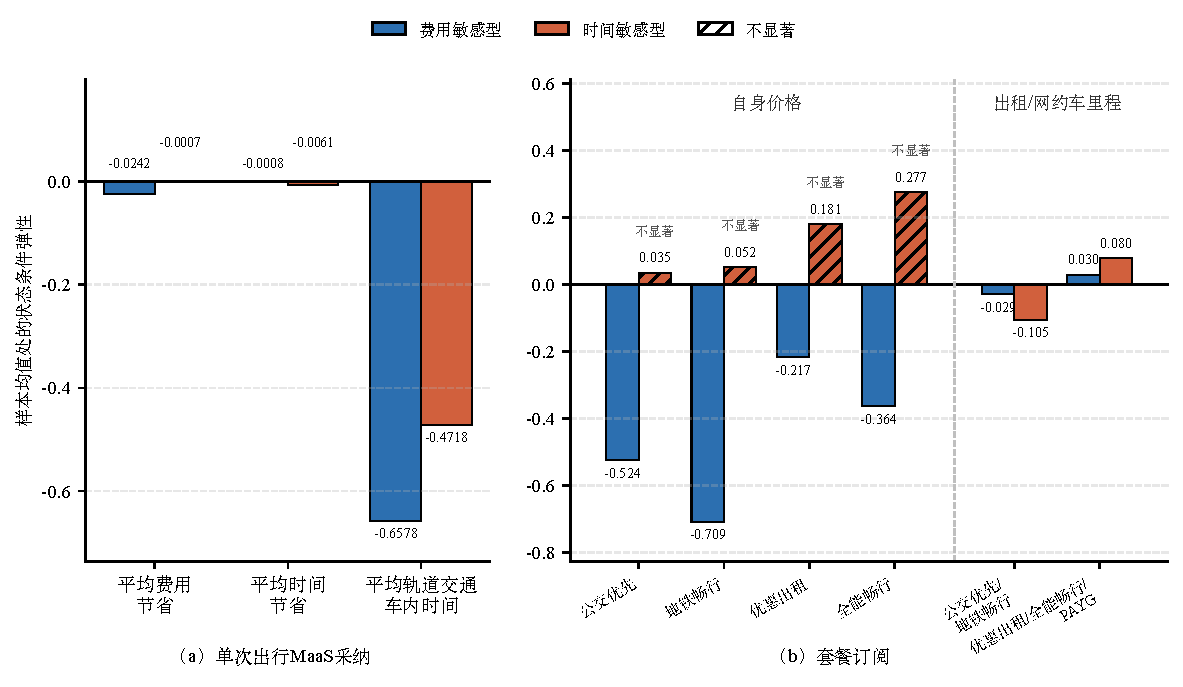
\includegraphics[width=\textwidth]{figures/ch6/中文版/elasticity_by_state.pdf}
  \bicaption{服务水平相关属性对MaaS多阶段采纳意愿的状态条件弹性}{State-conditional elasticities of multi-stage MaaS adoption intention with respect to level-of-service attributes.}
  \label{fig.int.elas.state}
\end{figure}

对于费用敏感型受访者，其决策主要取决于费用。在单次出行阶段，其转向MaaS多模式出行服务的意愿关于平均费用节省的弹性为$-0.024$，而关于平均时间节省的弹性仅为$-0.001$，即费用节省每改善1\%对费用敏感型采纳的提升约为时间节省的24倍；其关于MaaS选项平均轨道交通车内时间的弹性也较大（$-0.658$）。考虑到费用敏感型受访者在单次出行阶段中转向MaaS多模式出行服务的概率较低（21.7\%），因此，轨道服务水平的改善或许是针对此类受访者提高单次出行阶段MaaS采纳意愿的有效手段。在套餐订阅阶段，费用敏感型下四个价格弹性均为负且较大：公交优先$-0.524$、地铁畅行$-0.709$、优惠出租$-0.217$、全能畅行$-0.364$，其中两个公交导向套餐的价格敏感性更高，这可能因其更易被视为具有公交习惯的受访者的高性价比策略，价格变动对其性价比评估的影响更强。与之相对，公交导向套餐中可用的出租/网约车里程在该状态下的弹性几乎为零（公交优先与地铁畅行均为$-0.028$）。

对于时间敏感型受访者，其决策主要取决于时间。在单次出行阶段，其时间节省弹性为$-0.006$，约为费用敏感型的6倍，而费用节省弹性仅为$-0.001$。此外，轨道车内时间弹性为$-0.472$，量级小于费用敏感型，原因在于时间敏感型受访者的MaaS采纳概率很高（80.9\%），相同的影响系数所产生的采纳意愿的百分比变化更小。在套餐订阅阶段，时间敏感型的四个价格弹性均为正值（公交优先0.035、地铁畅行0.052、优惠出租0.181、全能畅行0.277）。究其原因，套餐价格并未进入时间敏感型受访者的决策考量，即该状态下套餐价格系数不显著（0.015）。故上述价格弹性应解读为零值附近的小幅响应，而非真实的行为结果。相比之下，价格系数的聚合弹性更能说明其对此类受访者的行为影响。套餐价格的整体上浮会使优惠出租与全能畅行的订阅份额分别下降0.167与0.121，同时使PAYG的订阅份额上升0.112。此外，公交导向套餐中可用的出租/网约车里程对时间敏感型受访者的弹性为$-0.105$（两套餐相同），量级约为费用敏感型的4倍，说明向公交导向套餐中加入出租车里程同样会抑制时间敏感型受访者的订阅。

综合以上两行为状态下的条件弹性结果，费用敏感型与时间敏感型不仅在行为偏好上不同，同一服务水平属性对采纳意愿的边际改善也呈现不同的特征，即费用敏感型受访者对费用类属性高度敏感、时间敏感型受访者对时间类属性高度敏感。然而，本节的状态条件弹性仅刻画了各状态对MaaS服务水平变化的响应，难以回答考虑全体用户的``哪些因素最能提升MaaS采纳''的问题，这正是下一小节的关注点。

\subsection{考虑全体用户的MaaS服务水平弹性}\label{subsec.int.disc.driver}

在理解不同行为状态下的受访者采纳MaaS的条件弹性后，MaaS运营方还需全面了解哪些因素最能提升全体潜在用户对MaaS的采纳意愿。为此，本节构建了从初始状态形成到套餐订阅的完整行为链条，并沿链条计算各因素对全体用户MaaS套餐订阅的聚合弹性，以作为MaaS长期发展的政策与运营干预的依据。具体而言，首先使用两种行为状态的初始分布与跨阶段转移概率，对状态条件弹性进行加权聚合，最终得到面向全体用户的聚合弹性。后续从MaaS套餐整体订阅弹性与分套餐的MaaS套餐订阅弹性两个角度进行分析。

\textbf{（1）MaaS套餐整体订阅弹性}

关于MaaS套餐整体订阅的聚合弹性如图~\ref{fig.int.elas.overall}所示。结果表明，MaaS多模式出行服务中的平均轨道交通车内时间的聚合弹性最大，为$-0.521$；平均费用节省与平均时间节省的聚合弹性分别约为$-0.014$与$-0.006$。状态转移过程中的套餐价格与受访者参照月度出行支出之间差异的聚合弹性为$-0.055$，公交导向套餐中可用的出租车/网约车里程为$-0.046$，各套餐价格的弹性则均低，均小于0.005。这说明MaaS多模式出行服务的平均轨道交通车内时间可能是提升潜在用户MaaS采纳意愿最有效的干预手段。

\begin{figure}[H]
  \centering
  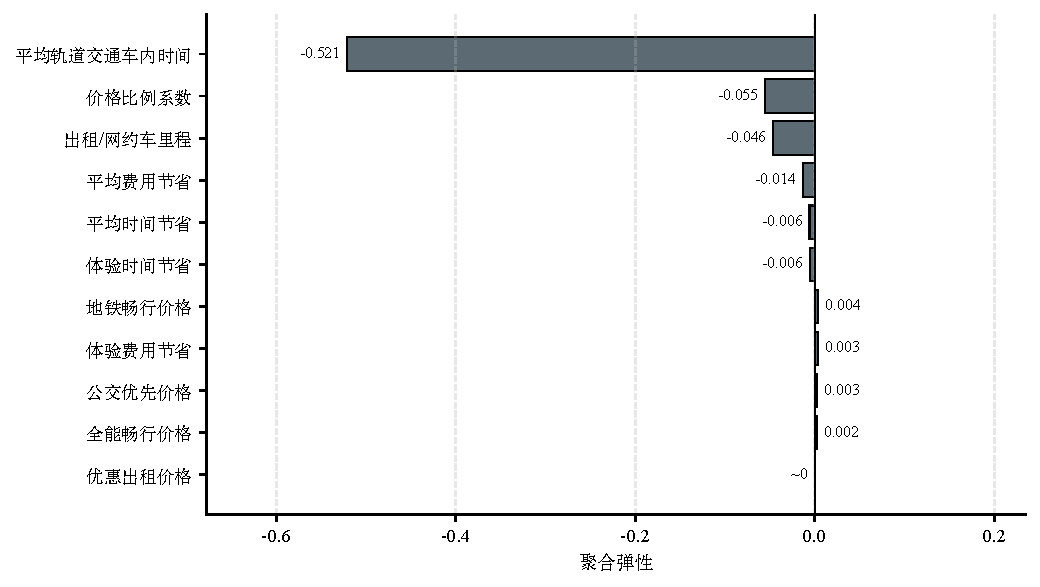
\includegraphics[width=\textwidth]{figures/ch6/中文版/elasticity_aggregate_overall.pdf}
  \bicaption{MaaS套餐整体订阅弹性}{Aggregate elasticities of overall MaaS bundle subscription.}
  \label{fig.int.elas.overall}
\end{figure}

\textbf{（2）分套餐的订阅弹性}

除MaaS套餐整体的订阅弹性外，对各套餐订阅概率的聚合弹性如图~\ref{fig.int.elas.bundle}所示。四个套餐的平均轨道交通车内时间、平均费用节省与平均时间节省弹性的规律近似，即关于平均轨道交通车内时间的弹性均为负且量级接近（公交优先$-0.519$、地铁畅行$-0.520$、优惠出租$-0.524$、全能畅行$-0.523$），关于费用节省与时间节省的弹性同样相似但量级较小（分别约$-0.014$与$-0.006$）。

在价格敏感性上，公交导向套餐和其他两类套餐的弹性计算结果呈现出两种不同的模式。对公交导向套餐，其对自身价格的聚合弹性较小（公交优先$-0.106$、地铁畅行$-0.183$），套餐所含的出租车/网约车里程会降低其订阅概率（公交优先$-0.081$、地铁畅行$-0.077$）。价格比例系数则弹性较小（公交优先0.013、地铁畅行$-0.005$），原因在于，公交导向套餐在两种行为状态下的订阅比例相近（公交优先为24.3\%对21.8\%，地铁畅行为32.4\%对23.3\%），价格比例系数变动所诱发的行为状态转移并不会导致套餐订阅结果的过多改变。此外，公交优先与地铁畅行二者之间的交叉价格弹性均为正（公交优先关于地铁畅行价格为0.087，反向为0.050），二者互为替代。与之相对，优惠出租与全能畅行对价格比例系数（分别$-0.167$与$-0.121$）与自身价格（分别$-0.178$与$-0.203$）均更为敏感。这一差异源于两状态下对这两种套餐的订阅份额分布，即费用敏感型状态下对优惠出租与全能畅行订阅意愿较大（集计后的订阅比例分别为23.4\%与17.6\%），而时间敏感型状态下的受访者几乎拒绝订阅这两类套餐（集计后的订阅比例分别为0.5\%与1.8\%）。此外，当价格比例系数上升时，受访者趋于转向时间敏感型，而时间敏感型状态下对这两类套餐的订阅意愿很低，其订阅比例随之下降。然而，优惠出租与全能畅行两类套餐可从公交导向套餐的价格变动中获得可观的替代需求，其关于公交优先套餐价格的交叉弹性分别为0.129与0.097，关于地铁畅行价格的交叉弹性分别为0.277与0.202，说明其会吸收费用敏感型受访者因公交导向套餐涨价而释放的套餐订阅需求。

\begin{figure}[H]
  \centering
  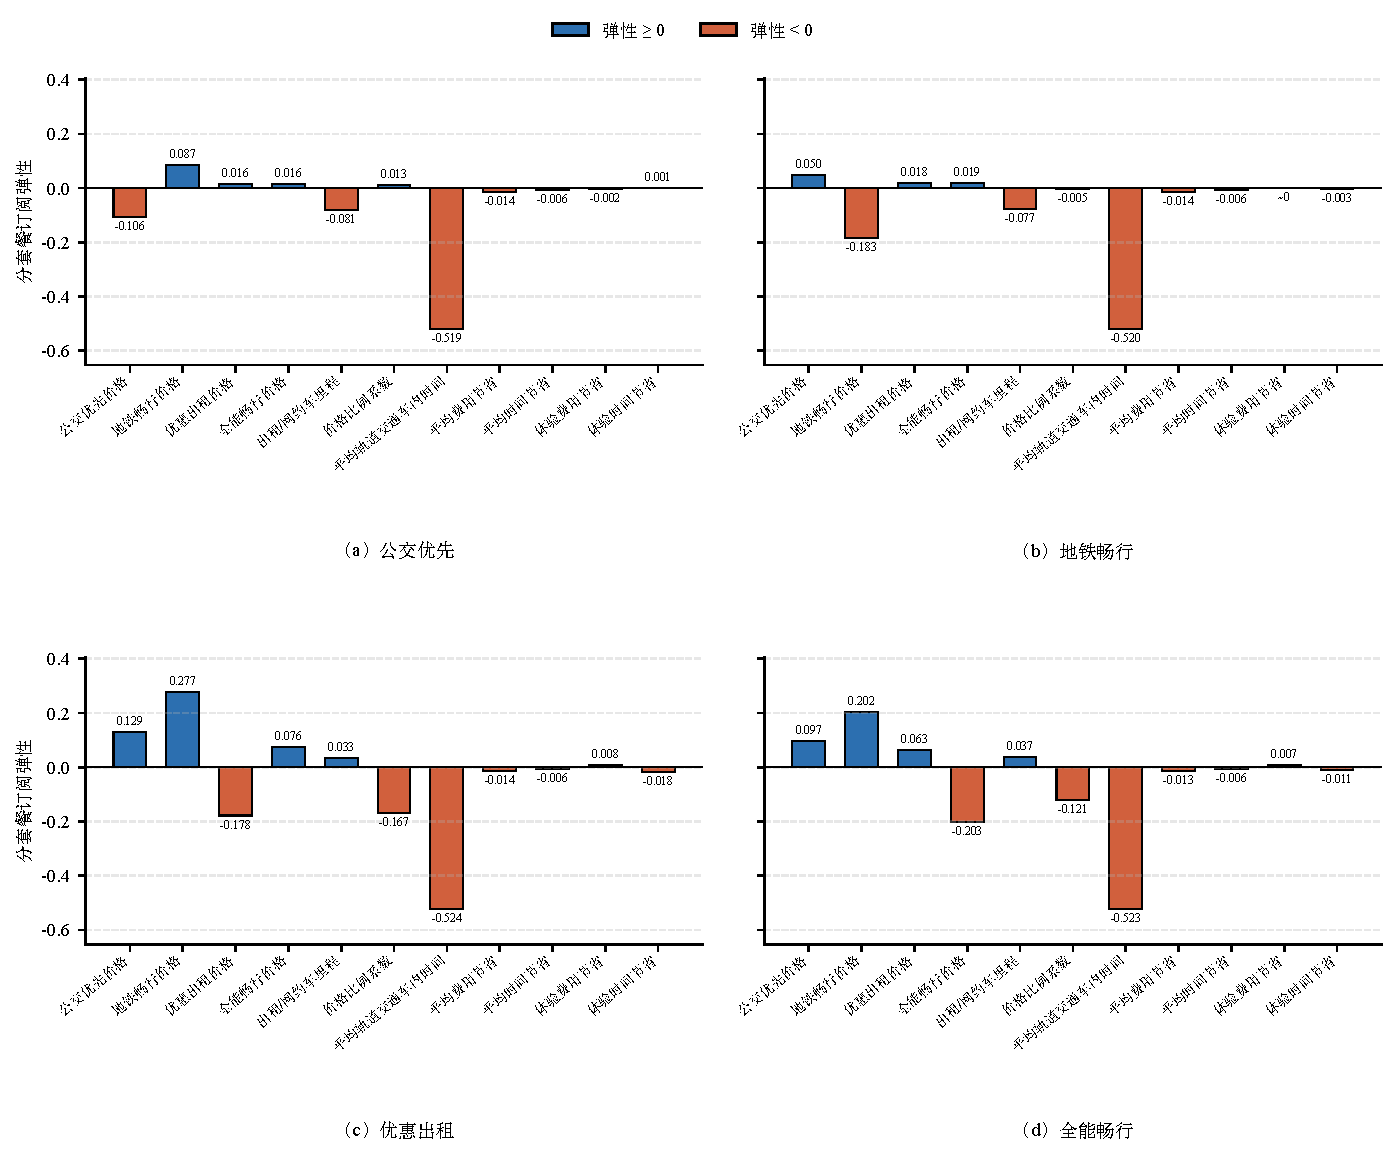
\includegraphics[width=\textwidth]{figures/ch6/中文版/elasticity_by_bundle.pdf}
  \bicaption{分套餐的订阅弹性}{Bundle-specific aggregate subscription elasticities.}
  \label{fig.int.elas.bundle}
\end{figure}

综上，单次出行阶段服务水平对最终套餐订阅的聚合弹性较大，尤其是MaaS多模式出行服务的平均轨道交通车内时间。在套餐订阅阶段，套餐内各属性的整体订阅弹性较小，因套餐内属性的调整主要导致受访者在四个套餐之间重新分配订阅需求，而非扩大套餐订阅总量。

\subsection{分阶段与一体化建模结果对比}\label{subsec.int.disc.compare}

在全面分析一体化建模视角下得到的结果后，本小节进一步针对第\ref{chap.staged}章的分阶段建模结果与本章的一体化建模结果进行对比，有助于厘清两种建模方法的适用边界，并为第\ref{chap.optimization}章的行为参数选用奠定基础。

\textbf{（1）共同发现}

就实质结论而言，两种建模视角相互印证了若干结论：其一，受访者的MaaS偏好高度异质；其二，货币成本是核心决策驱动；其三，公共交通用户较私家车用户更易接受MaaS。此外，既有研究中关于社会经济属性的规律性结论，即女性、较高收入者、高受教育程度者与技术热衷者更易接受MaaS，在本章估计中同样得到确认。在此之上，一体化建模还揭示了分阶段建模难以呈现的细节。例如，经常乘坐地铁的受访者倾向于初始归属于时间敏感型状态，而经常乘坐公交的受访者则倾向于初始归属于费用敏感型状态，即``公交用户更易接受MaaS''这一结论存在公交用户与地铁用户的分化，有助于运营方区分应优先瞄准的公交细分人群。

\textbf{（2）方法论差异}

两种建模方法的差异主要体现在两方面。

其一是异质性的处理方式。分阶段建模通过潜在分类刻画行为异质性，受访者的潜在类型在各阶段内固定不变；一体化建模则通过HMM允许行为状态在单次出行与套餐订阅两阶段间转移，从而观测到分阶段建模设定无法捕捉的状态转移机理，例如，在单次出行阶段体验到的MaaS多模式出行服务节省的费用将使受访者更倾向于转入费用敏感型状态，节省的时间将使其更倾向于转向时间敏感型状态。

其二是跨阶段的衔接方式。分阶段建模以单次出行阶段计算得到的转移意愿指数衔接两阶段，并先后独立估计两阶段的选择模型；一体化建模则在单一联合似然下、经$K^2$条状态路径求和同时估计两阶段行为选择。正是凭借这一联合结构，本章得以量化单次出行阶段属性对最终套餐订阅的整体影响。

\textbf{（3）适用边界}

综合而言，两种建模视角各有其适用情境。分阶段建模的优势在于，可在各阶段内引入更丰富的模型结构（如套餐订阅阶段的属性无视、嵌套Logit巢结构与精细的潜在类别画像），从而分别精细刻画两阶段的偏好异质性，各阶段的行为可解释性更强，适于面向单一阶段、需要精细划分人群画像的运行需求。一体化建模的优势则在于，在统一似然函数下联合刻画初始状态形成、跨阶段状态转移与两阶段选择，能够直接捕捉单次出行获取到的出行体验对套餐偏好的影响，并在全周期视角下给出MaaS采纳的关键因素，适于理解跨阶段的动态联系与全生命周期的MaaS采纳意愿。

%==================================================================
\section{本章小结}\label{sec.int.summary}

本章在第\ref{chap.staged}章分阶段建模的基础上，研究了一体化建模视角下的MaaS多阶段采纳意愿建模问题。针对分阶段建模无法捕捉受访者从单次出行到套餐订阅阶段的行为状态转移、难以通过统一的建模方式刻画受访者全过程采纳意愿的局限性，本章提出了结合MIMIC模型的HMM建模框架，完整地刻画了受访者从初始状态形成、单次出行选择、跨阶段状态转移到套餐订阅选择的全过程，并经与第\ref{chap.staged}章相同的两步式SP调查数据（1242份有效样本）加以标定与验证。主要工作与结论如下。

其一，构建了MIMIC-HMM建模框架。该框架通过MIMIC模型从态度陈述中计算五个态度潜变量的态度得分，并将其纳入初始行为状态的形成过程。进一步，构建HMM模型在联合刻画初始行为状态形成、单次出行选择、跨阶段状态转移与套餐订阅选择四个相互衔接的过程，并构建统一的似然函数。Biogeme标定结果表明，调整后McFadden $\rho^2$达0.200，表明HMM模型对受访者MaaS多阶段采纳意愿的拟合良好。

其二，识别出两种具有显著偏好异质性的行为状态。通过对受访者多阶段MaaS采纳行为的一体化估计，HMM识别出贯穿受访者决策行为全周期的费用敏感型与时间敏感型两个状态，分别占初始状态分布的63.4\%与36.6\%，反映受访者以费用或以时间为先的两类决策偏好。在单次出行阶段，费用敏感型受访者对MaaS多模式出行服务带来的费用节省敏感，而时间敏感型受访者对则更关注单次出行中MaaS多模式出行服务的时间成本；在套餐订阅阶段，费用敏感型受访者偏好公交导向套餐且对价格高度敏感，时间敏感型受访者则偏好PAYG（占其订阅的52.6\%），但对能满足其出行需求的套餐仍有一定的订阅意愿。

其三，揭示了跨阶段行为状态转移机理。在单次出行阶段体验到更高MaaS多模式出行服务带来的费用节省的受访者更可能转入或保持费用敏感型状态，体验到更高MaaS多模式出行服务带来的时间节省的受访者则更可能转入时间敏感型状态；套餐价格偏离当前每月的出行成本、套餐的价格比例系数偏高均会使受访者不再保持费用敏感型状态。这一机理刻画了既有文献与第\ref{chap.staged}章所未能捕捉的、连接``初次体验''与``长期订阅''的动态行为状态转换。

其四，给出了从单次出行到套餐订阅全周期的MaaS采纳关键因素。沿``初始状态$\rightarrow$单次出行$\rightarrow$状态转移$\rightarrow$套餐订阅''的行为链条的聚合弹性表明，单次出行阶段MaaS多模式出行服务的平均轨道交通车内时间聚合弹性最大，为$-0.521$，比所有套餐内服务水平属性的聚合弹性均高出一个数量级。此外，单次出行阶段的MaaS多模式出行服务的平均费用节省与时间节省也具有较高的聚合弹性，而套餐内的价格与出租/网约车里程的聚合弹性均较小。以上针对全体用户的聚合弹性分析为MaaS全生命周期推广策略提供了行为依据。

上述分阶段建模与一体化建模的结果各有侧重、相互补充：第\ref{chap.staged}章分阶段建模可获得各阶段的选择模型与各阶段内精细的人群画像，有助于理解各阶段的行为偏好与异质性；本章一体化建模则可刻画跨阶段的行为状态转移机理，所得的全周期MaaS采纳关键因素的聚合弹性分析，则为推广策略着力点提供了行为层面的依据。
